
\documentclass[12pt]{exam}
\usepackage{amsthm}
\usepackage{libertine}
%\usepackage[utf8]{inputenc}
\usepackage[margin=1in]{geometry}
\usepackage{amsmath,amssymb}
\usepackage{multicol}
\usepackage[shortlabels]{enumitem}
\usepackage{siunitx}
\usepackage{cancel}
\usepackage{graphicx}
\graphicspath{{./}}
\usepackage{pgfplots}
\usepackage{hyperref}
\usepackage{listings}
\usepackage{tikz}
\usepackage{minted}
\def\code#1{\texttt{#1}}
\usepackage{amssymb}
\usepackage{xcolor}
% for plotting
\usepackage{pgfplots}
\pgfplotsset{compat=1.16}
\usepackage{tikz}
\usetikzlibrary{arrows.meta}

\newcommand{\quotebox}[1]
{
  \begin{center}
    \fcolorbox{white}{blue!15!gray!15}{
      \begin{minipage}{0.7\linewidth}\vspace{10pt}
        \center
        \begin{minipage}{0.8\linewidth}{\space\Huge``}{\setlength{\parindent}{1.5em}#1}{\hspace{1.5em}\break\null\Huge\hfill''}
        \end{minipage}
        \smallbreak
      \end{minipage}
    }
\end{center}
}

%\DeclareUnicodeCharacter{2212}{-}


\let\oldemptyset\emptyset
\let\emptyset\varnothing

\hypersetup{
    colorlinks=true,
    linkcolor=blue,
    filecolor=magenta,      
    urlcolor=cyan,
    pdftitle={Overleaf Example},
    pdfpagemode=FullScreen,
    }
    
\urlstyle{same}

\pgfplotsset{width=10cm,compat=1.9}
\usepgfplotslibrary{external}
\tikzexternalize

\newcommand{\class}{Math 415} % This is the name of the course 
\newcommand{\examnum}{Homework-5} % This is the name of the assignment
\newcommand{\examdate}{Oct 18} % This is the due date
\newcommand{\timelimit}{}

\newcommand{\BO}{\mathcal{O}}




\begin{document}
\pagestyle{plain}
\thispagestyle{empty}

\noindent
\begin{tabular*}{\textwidth}{l @{\extracolsep{\fill}} r @{\extracolsep{6pt}} l}
\textbf{\class} & \textbf{Name:} & \textit{Zhenzhao Tu}\\ %Your name here instead, obviously 
\textbf{\examnum} &&\\
\textbf{\examdate} &&\\
\end{tabular*}\\
\rule[2ex]{\textwidth}{2pt}
% --

\section*{Problem 1}
Decide the origin if is attractting, Lyapunov stable, asymptotically stable, or none of them.

\begin{enumerate}[(a)]
    \item $\dot{x} = y , \quad \dot{y} = -4x$
	    The Jacobian matrix is
	    \[ J = \begin{bmatrix}
	        0 & 1 \\
	        -4 & 0 \\
		\end{bmatrix} , \quad \lambda = \pm 2i, \quad v_1= \begin{bmatrix}
		    -i \\
		    2 \\
		\end{bmatrix} , \quad v_2 = \begin{bmatrix}
		i \\
		2 \\
		\end{bmatrix} \]
	The node is center. The origin is Lyapunov stable.

    \item $\dot{x} = 2y, \quad \dot{y} = x$
	    The Jacobian matrix is
	    \[ J = \begin{bmatrix}
	        0 & 2 \\
	        1 & 0 \\
		\end{bmatrix} , \quad \lambda = \pm \sqrt{2}, \quad v_1= \begin{bmatrix}
		-\sqrt{2} \\
		1 \\
		\end{bmatrix} , \quad v_2 = \begin{bmatrix}
		\sqrt{2} \\
		1 \\
		\end{bmatrix} \]
   	The node is a saddle node. The origin is none of them. 

    \item $\dot{x} = x-y, \quad \dot{y} = x+y$
	    The Jacobian matrix is
	    \[ J = \begin{bmatrix}
	        1 & -1 \\
	        1 & 1 \\
		\end{bmatrix} , \quad \lambda = 1\pm i , \quad v_1= \begin{bmatrix}
		i \\
		1 \\
		\end{bmatrix} , \quad v_2 = \begin{bmatrix}
		-i \\
		1 \\
	\end{bmatrix} \]

	The node is center, but it is repelling. The origin is none of them.

    \item $\dot{x} = 0, \quad \dot{y} = -y$
	    The Jacobian matrix is
	    \[ J = \begin{bmatrix}
	        0 & 0 \\
	        0 & -1 \\
		\end{bmatrix} , \quad \lambda = 0, -1 , \quad v_1= \begin{bmatrix}
		0 \\
		1 \\
		\end{bmatrix} , \quad v_2 = \begin{bmatrix}
		1 \\
		0 \\
	\end{bmatrix} \]
	The node is non-isolated. The origin is Lyapunov stable but not attracting, so it is Neutrally stable.

     \item $ \dot{x} = -x, \quad \dot{y} = -5y$
	    The Jacobian matrix is
	    \[ J = \begin{bmatrix}
	        -1 & 0 \\
	        0 & -5 \\
		\end{bmatrix} , \quad \lambda = -1, -5 , \quad v_1= \begin{bmatrix}
		1 \\
		0 \\
		\end{bmatrix} , \quad v_2 = \begin{bmatrix}
		0 \\
		1 \\
	\end{bmatrix} \]
	
	The node is stable node. The origin is globally asymptotically stable.

    \item $\dot{x} = x, \quad \dot{y} = y$
	    The Jacobian matrix is
	    \[ J = \begin{bmatrix}
	        1 & 0 \\
	        0 & 1 \\
		\end{bmatrix} , \quad \lambda = 1, 1 , \quad v_1= \begin{bmatrix}
		1 \\
		0 \\
		\end{bmatrix} , \quad v_2 = \begin{bmatrix}
		0 \\
		1 \\
	\end{bmatrix} \]

	This node is star but unstable. The origin is none of them.

\end{enumerate}

\section*{Problem 2}
Consider several systems then first find the Jacobian matrix and eigenunit, then find the final solution of the system. Last,classify the origin then plot the phase portrait.

\begin{enumerate}[(a)]
	\item $\dot{x} = 4x-y, \quad \dot{y}=2x+y$
	
	The Jacobian matrix is
	\[ J = \begin{bmatrix}
		4 & -1 \\
		2 & 1 \\
	\end{bmatrix} , \quad \lambda = 3, 2 , \quad v_1= \begin{bmatrix}
	1 \\
	1 \\
	\end{bmatrix} , \quad v_2 = \begin{bmatrix}
	1 \\
	2 \\
	\end{bmatrix} \]

	The general solution is
	\[ x(t) = c_1e^{3t} \begin{bmatrix}
		1 \\
		1 \\
	\end{bmatrix} + c_2e^{2t} \begin{bmatrix}
		1 \\
		2 \\
	\end{bmatrix} \]

	The origin is unstable node. The phase portrait is
	%put image to left of text
	\begin{figure}[h]
		\centering
		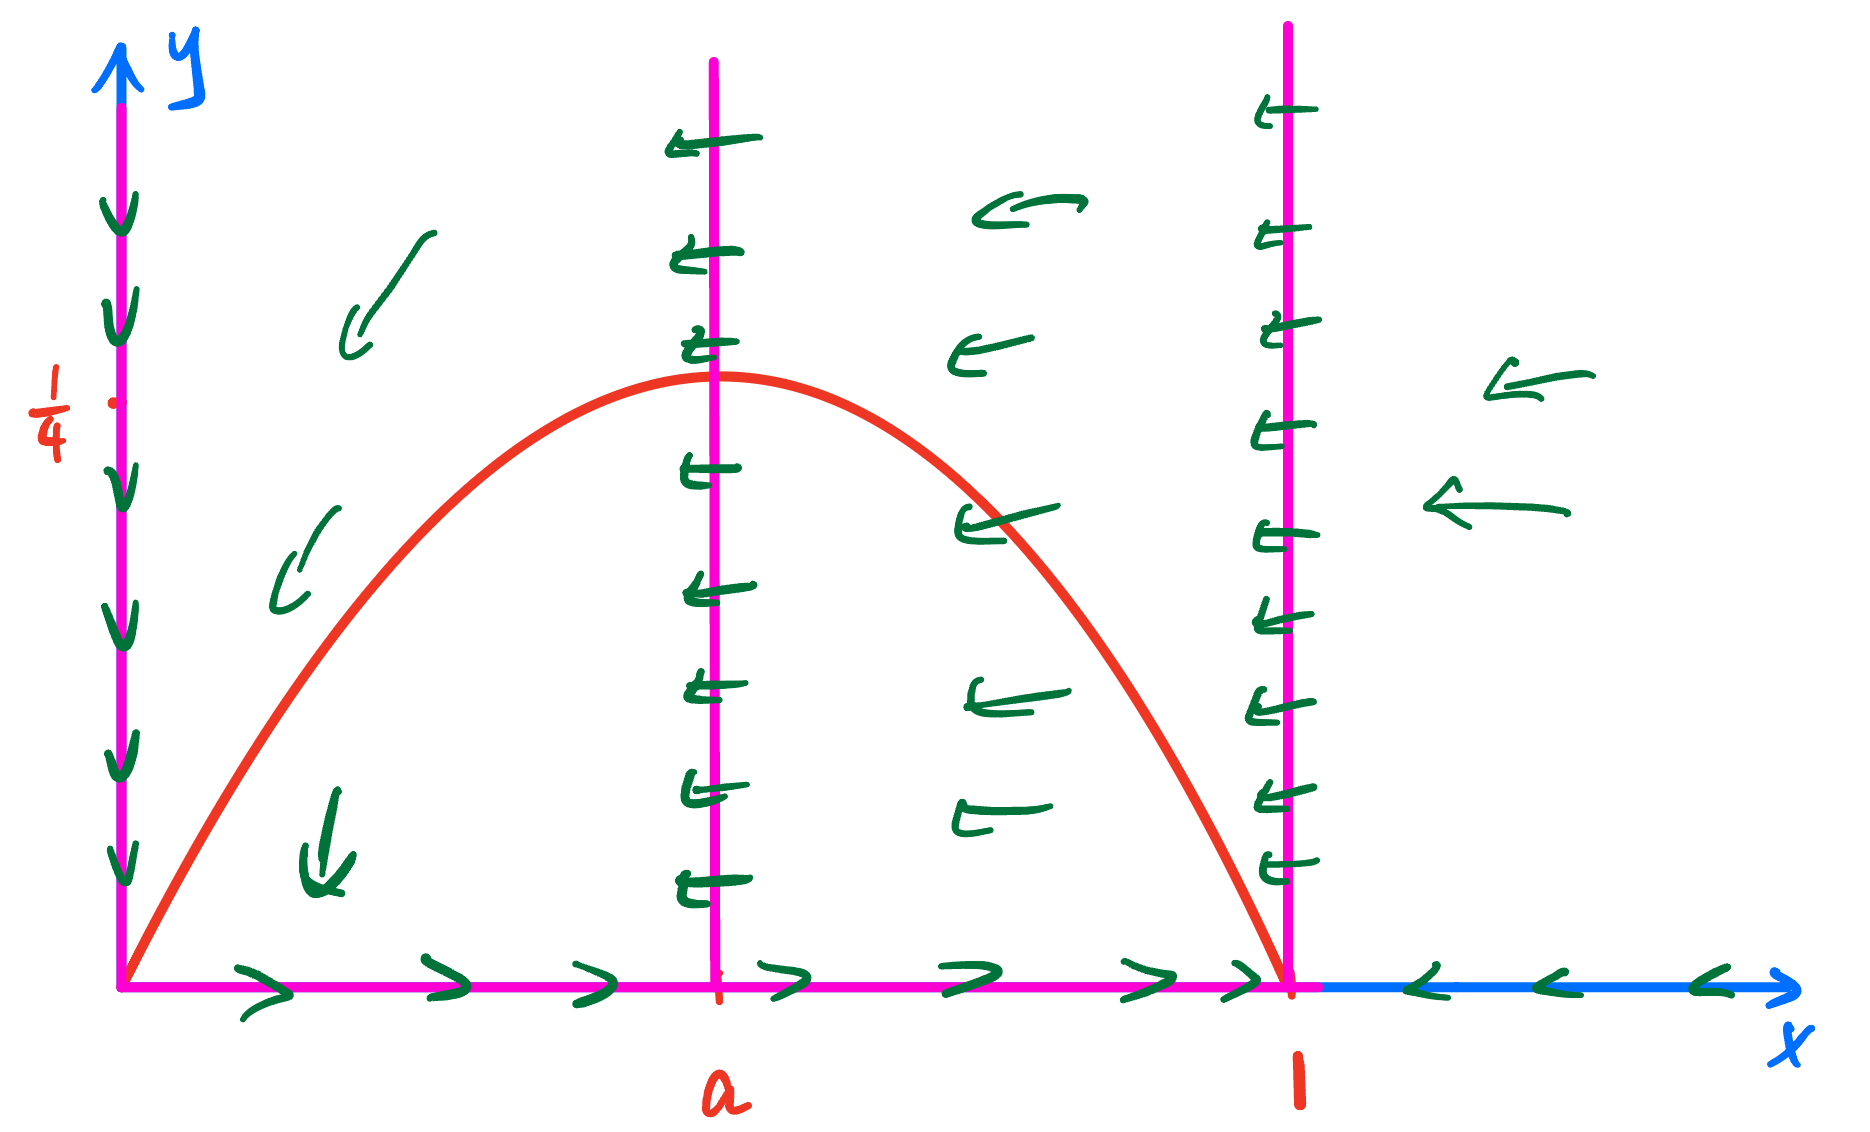
\includegraphics[width=0.6\linewidth]{2a.jpeg}
		\caption{Phase portrait of (a)}
		\label{fig:2a}
	
	\end{figure}

	\item $\dot{x} = x-y, \dot{y} = x+y$

	The Jacobian matrix is
	\[ J = \begin{bmatrix}
		1 & -1 \\
		1 & 1 \\
	\end{bmatrix} , \quad \lambda = 1\pm i , \quad v_1= \begin{bmatrix}
	i \\
	1 \\
	\end{bmatrix} , \quad v_2 = \begin{bmatrix}
	-i \\
	1 \\
	\end{bmatrix} \]

	The general solution is
	\[ x(t) = c_1e^{1+it} \begin{bmatrix}
		i \\
		1 \\
		\end{bmatrix} + c_2e^{1-it} \begin{bmatrix}
	-i \\
	1 \\
	\end{bmatrix} \]
	
	The origin is center but repelling. The phase portrait is

	\begin{figure}[H]
		\centering
		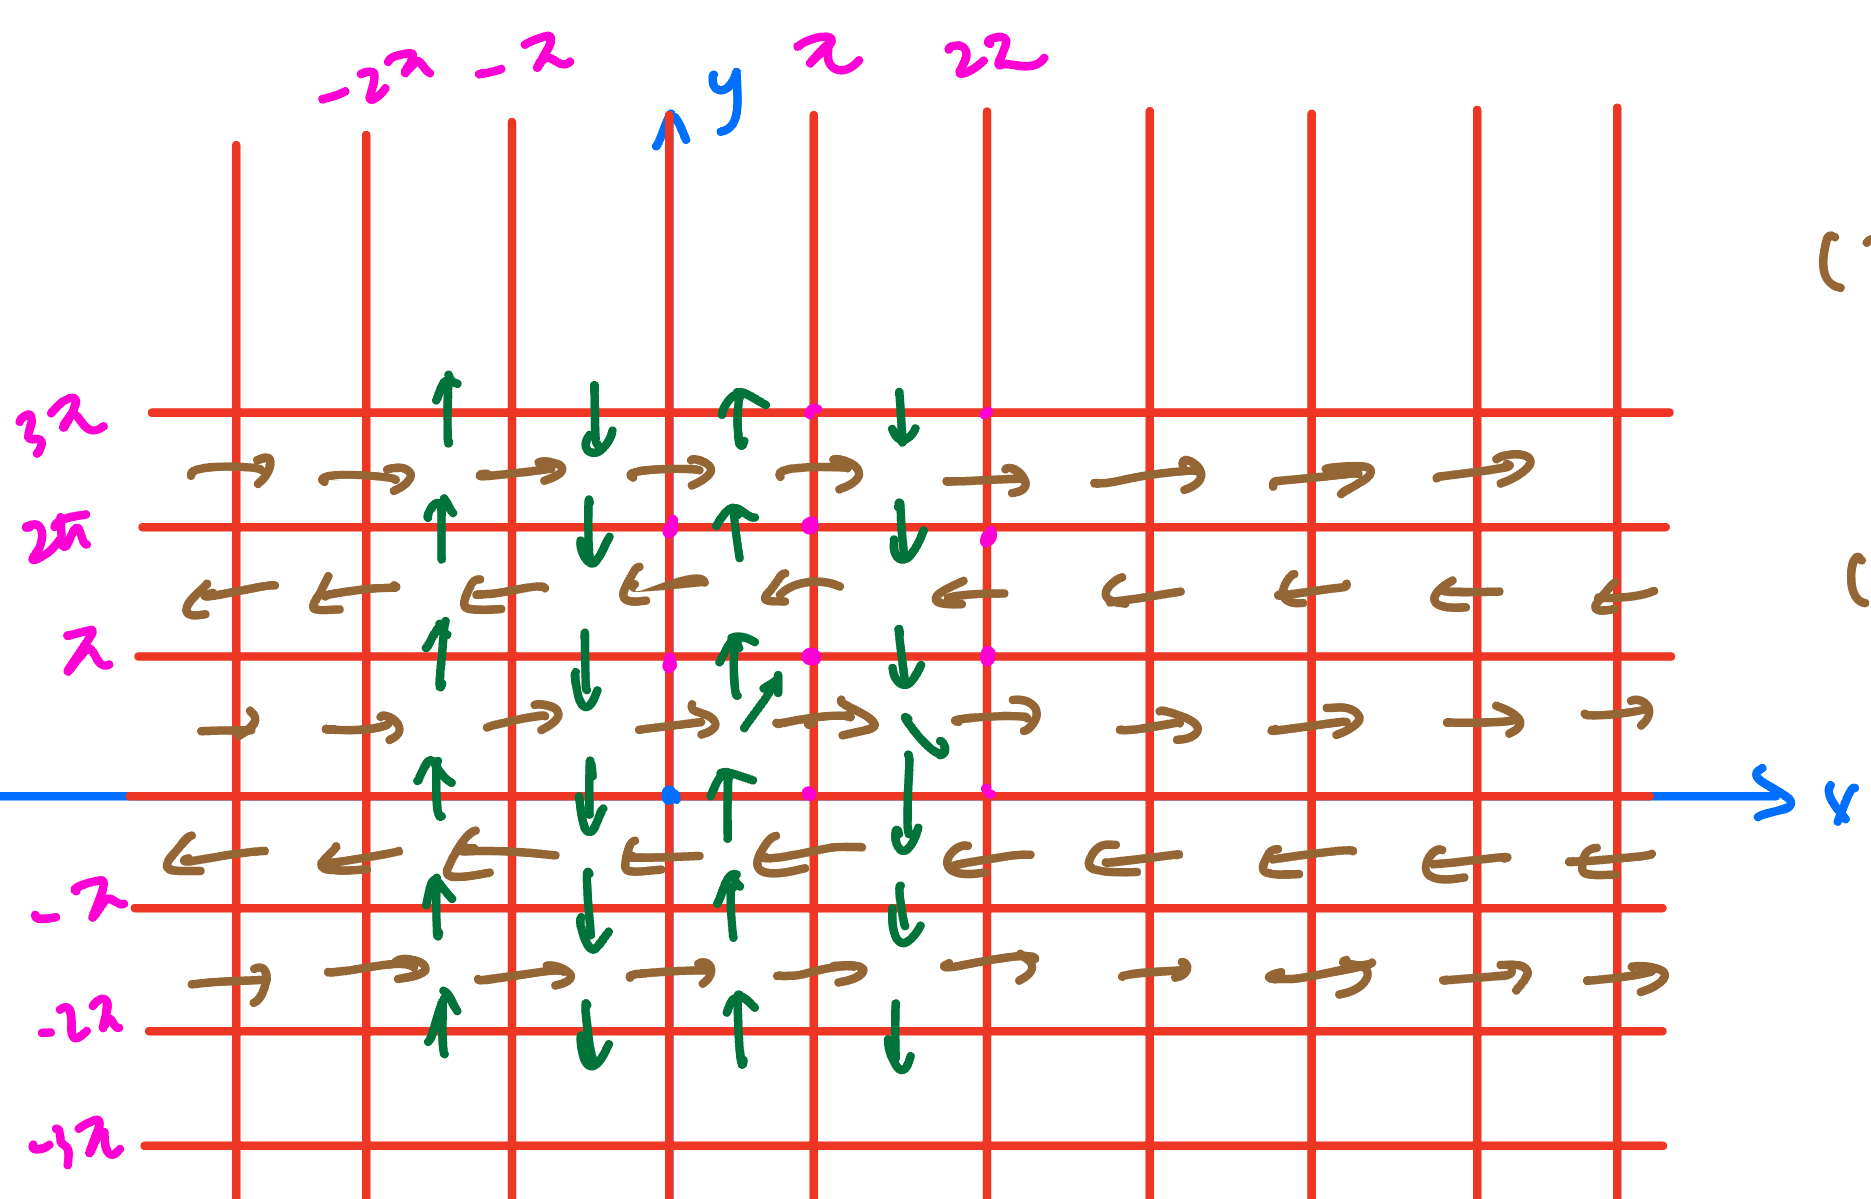
\includegraphics[width=0.6\linewidth]{2b.jpeg}
		\caption{Phase portrait of (b)}
		\label{fig:2b}
	\end{figure}

	\item $\dot{x} = 4x-3y, \quad \dot{y} = 8x-6y$

	The Jacobian matrix is
	\[ J = \begin{bmatrix}
		4 & -3 \\
		8 & -6 \\
	\end{bmatrix} , \quad \lambda = 0, -2 , \quad v_1= \begin{bmatrix}
	1 \\
	2 \\
	\end{bmatrix} , \quad v_2 = \begin{bmatrix}
	3 \\
	4 \\
	\end{bmatrix} \]

	The general solution is
	\[ x(t) = c_1e^{-2t} \begin{bmatrix}
		1 \\
		2 \\
		\end{bmatrix} + c_2 \begin{bmatrix}
		3 \\
		4 \\
		\end{bmatrix} \]
	
	The origin is degenerate node. The phase portrait is

	\begin{figure}[H]
		\centering
		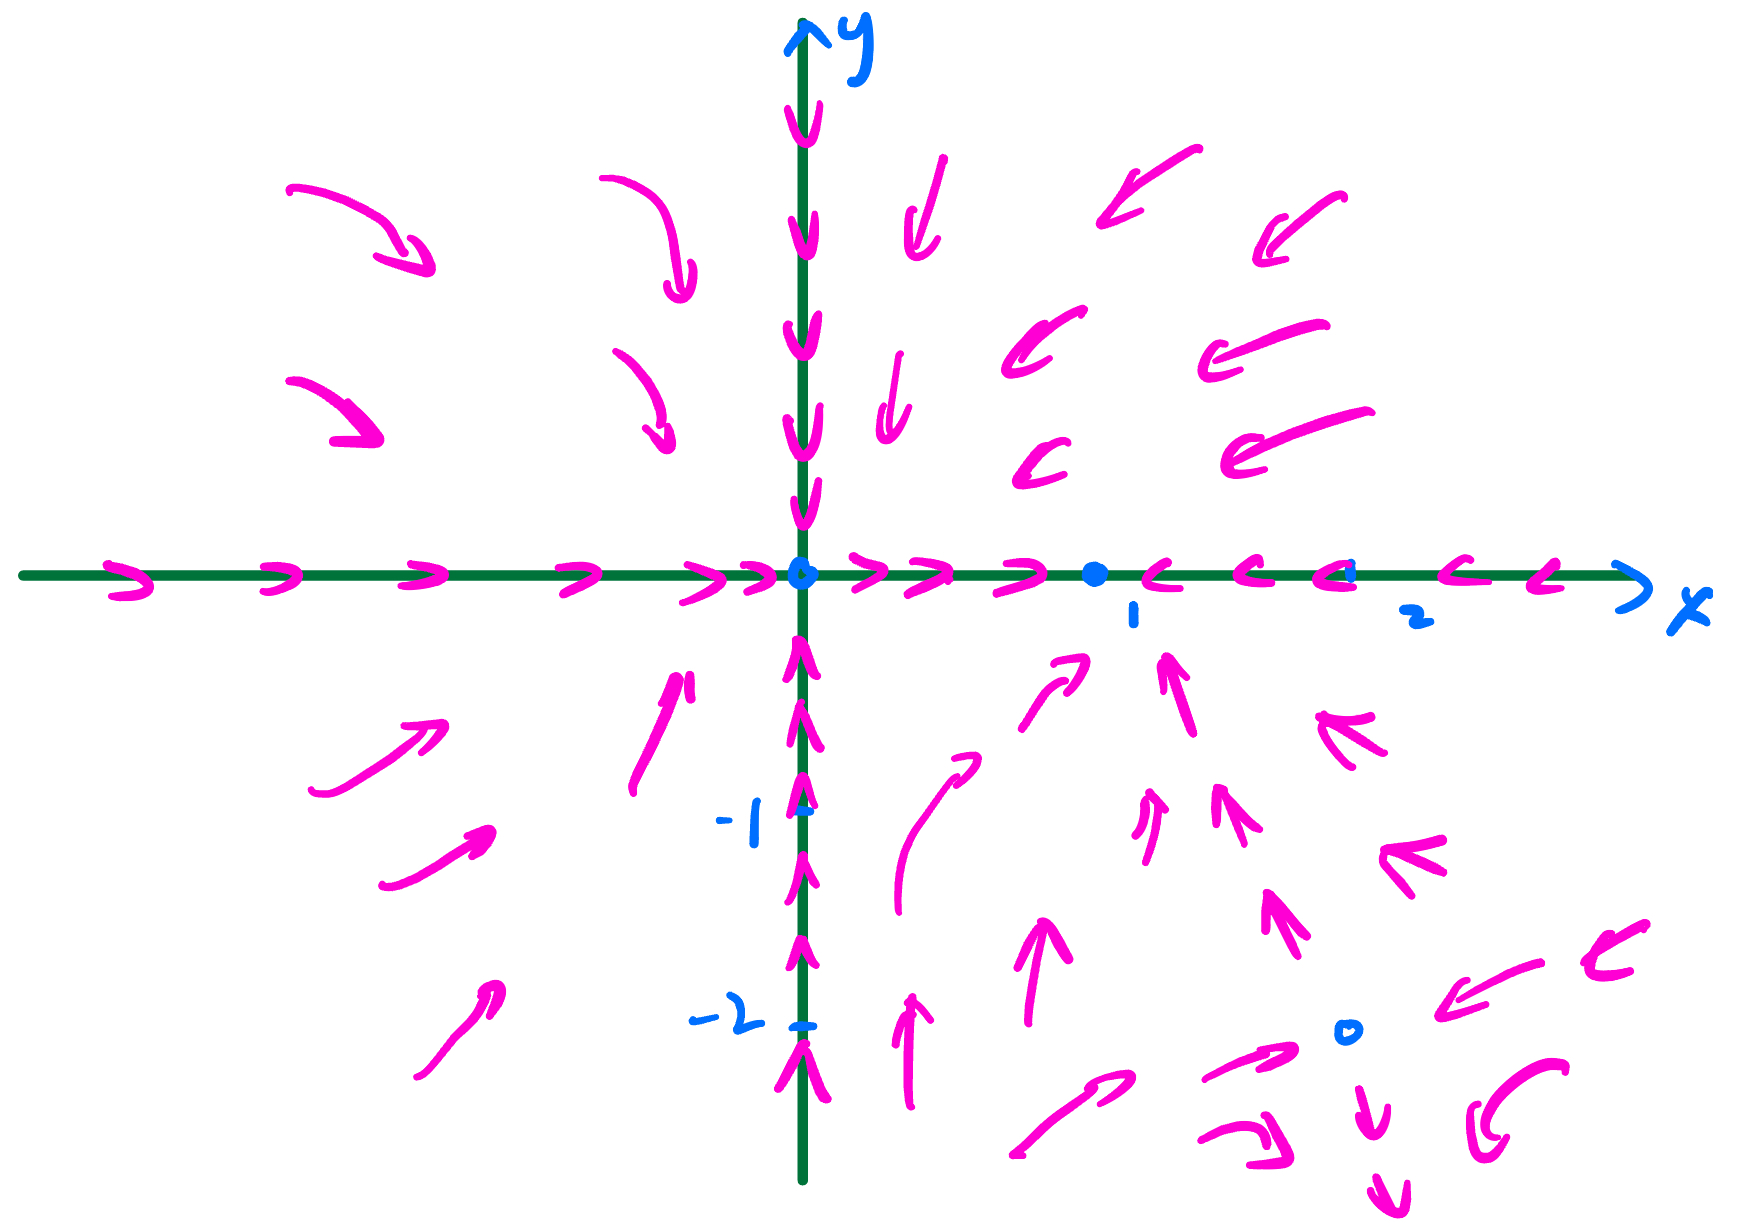
\includegraphics[width=0.6\linewidth]{2c.jpeg}
		\caption{Phase portrait of (c)}
		\label{fig:2c}
	\end{figure}

	\item $\dot{x} = 5x+2y, \quad \dot{y} = -17x-5y$
	
	The Jacobian matrix is
	\[ J = \begin{bmatrix}
		5 & 2 \\
		-17 & -5 \\
	\end{bmatrix} , \quad \lambda = \pm 3i , \quad v_1= \begin{bmatrix}
	-5-3i \\
	17 \\
	\end{bmatrix} , \quad v_2 = \begin{bmatrix}
	-5+3i \\
	17 \\
	\end{bmatrix} \]

	The general solution is
	\[ x(t) = c_1e^{3it} \begin{bmatrix}
		-5-3i \\
		17 \\
		\end{bmatrix} + c_2e^{-3it} \begin{bmatrix}
		-5+3i \\
		17 \\
		\end{bmatrix} \]
	
	The origin is center and attracting. The phase portrait is

	\begin{figure}[H]
		\centering
		\includegraphics[width=0.6\linewidth]{2d.jpeg}
		\caption{Phase portrait of (d)}
		\label{fig:2d}
	\end{figure}


\end{enumerate}

\section*{Problem 3}

For $A = \begin{bmatrix}
	\lambda & b \\
	0 & \lambda \\
\end{bmatrix}$, the eigenvalue is $\lambda$ and $b \not= 0$. Consider the characteristic equation of $A$, we have
\[(A-\lambda I)\mathbf{v} = \begin{bmatrix}
	\lambda - \lambda & b \\
	0 & \lambda - \lambda \\
	\end{bmatrix} = \begin{bmatrix}
	0 & b \\
	0 & 0 \\
	\end{bmatrix} \mathbf{v} = \mathbf{0} \]

	So, the system of equations is
	\[ \begin{cases}
		0v_1 + bv_2 = 0 \\
		0v_1 + 0v_2 = 0 \\
	\end{cases} \]

	From the equations we can see that the eigenvector $(1,0)$ is dependent on $b$, and since $b \not= 0$, the $v_2$ must be zero. Therefore, we have shown that there is only one eigenvector corresponding to the eigenvalue $\lambda$.

	So, when $\lambda, b < 0$ the origin is asymptotically stable. The phase portrais below:
	\begin{figure}[H]
		\centering
		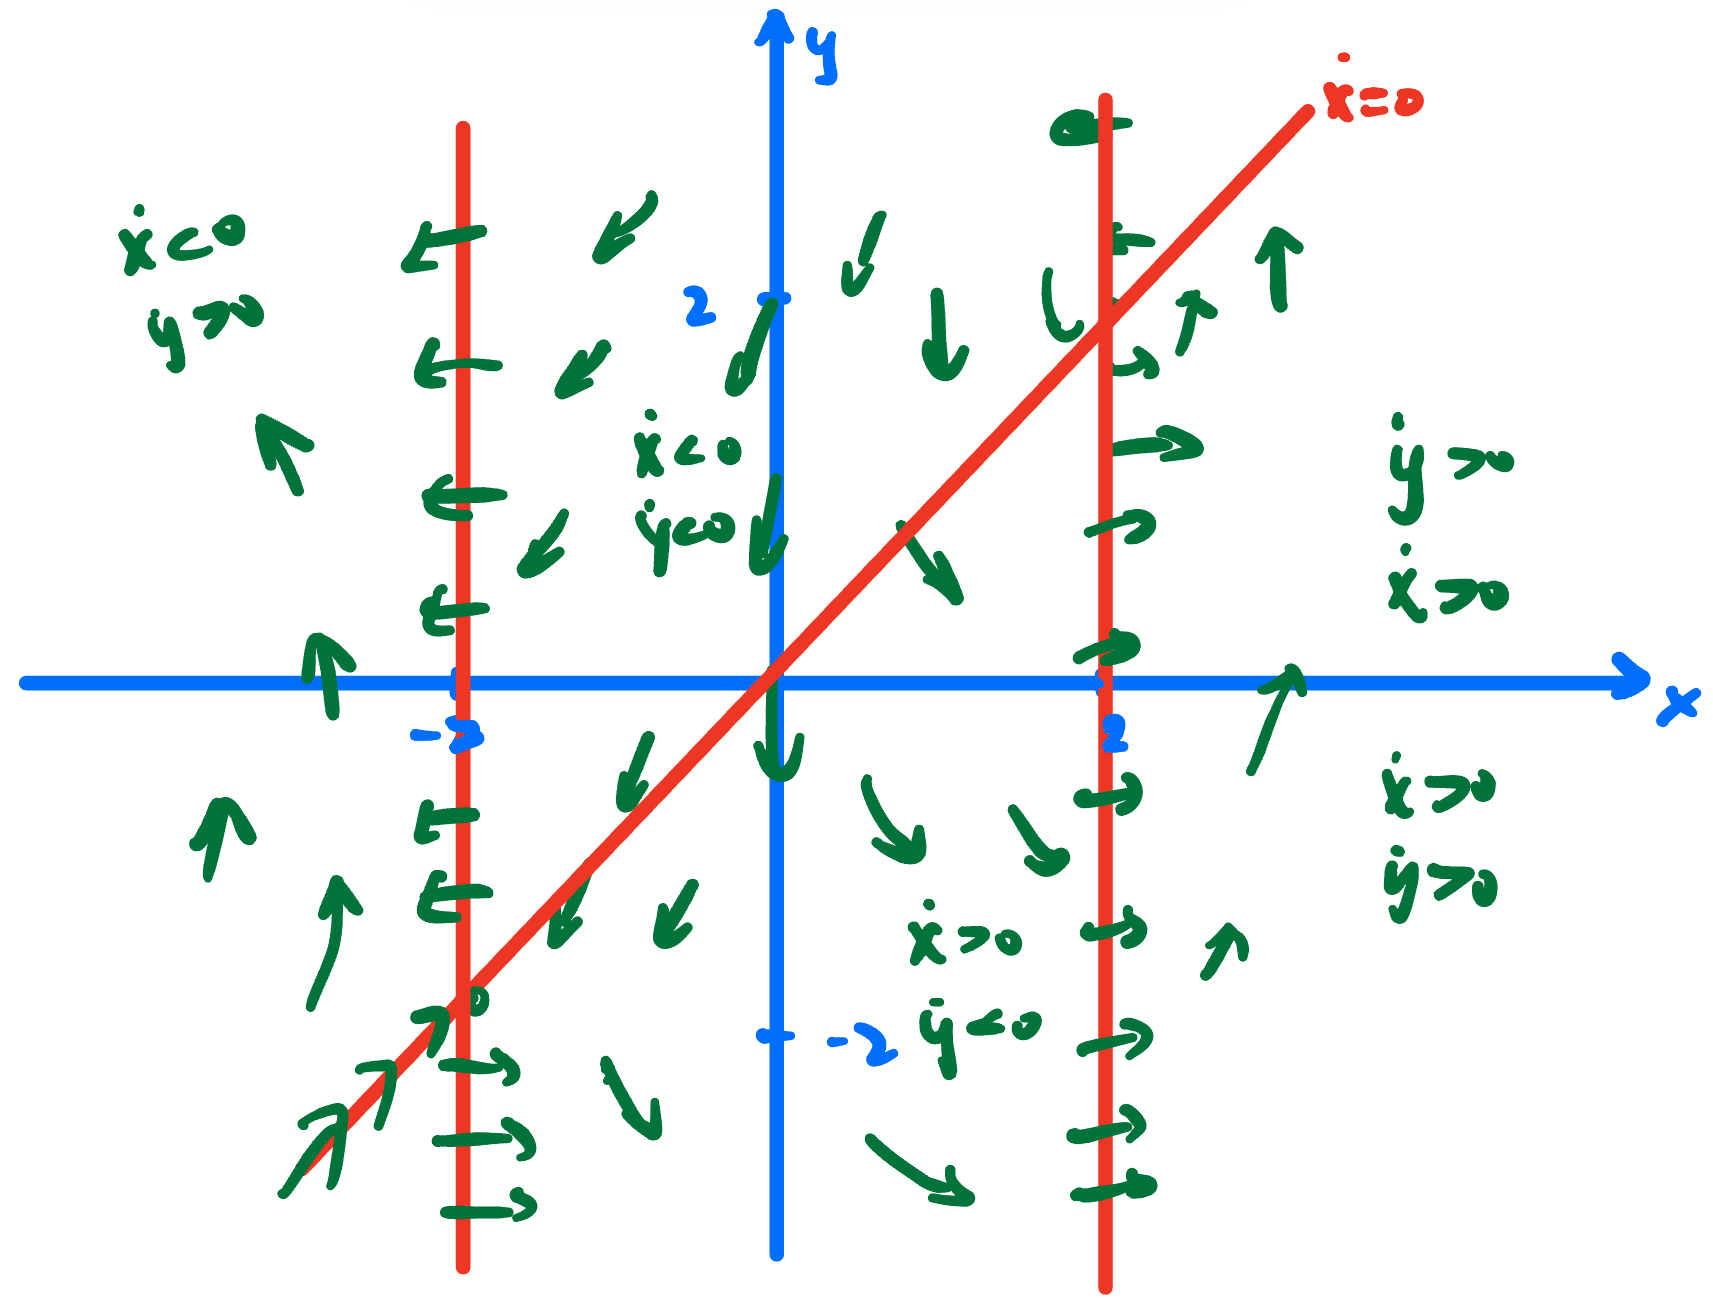
\includegraphics[width=0.7\linewidth]{3a.jpeg}
		\caption{Phase portrait of (a)}
		\label{fig:3a}
	\end{figure}

	When $\lambda <0 <b$, the origin is also asymptotically stable. The phase portrais below:
	\begin{figure}[H]
		\centering
		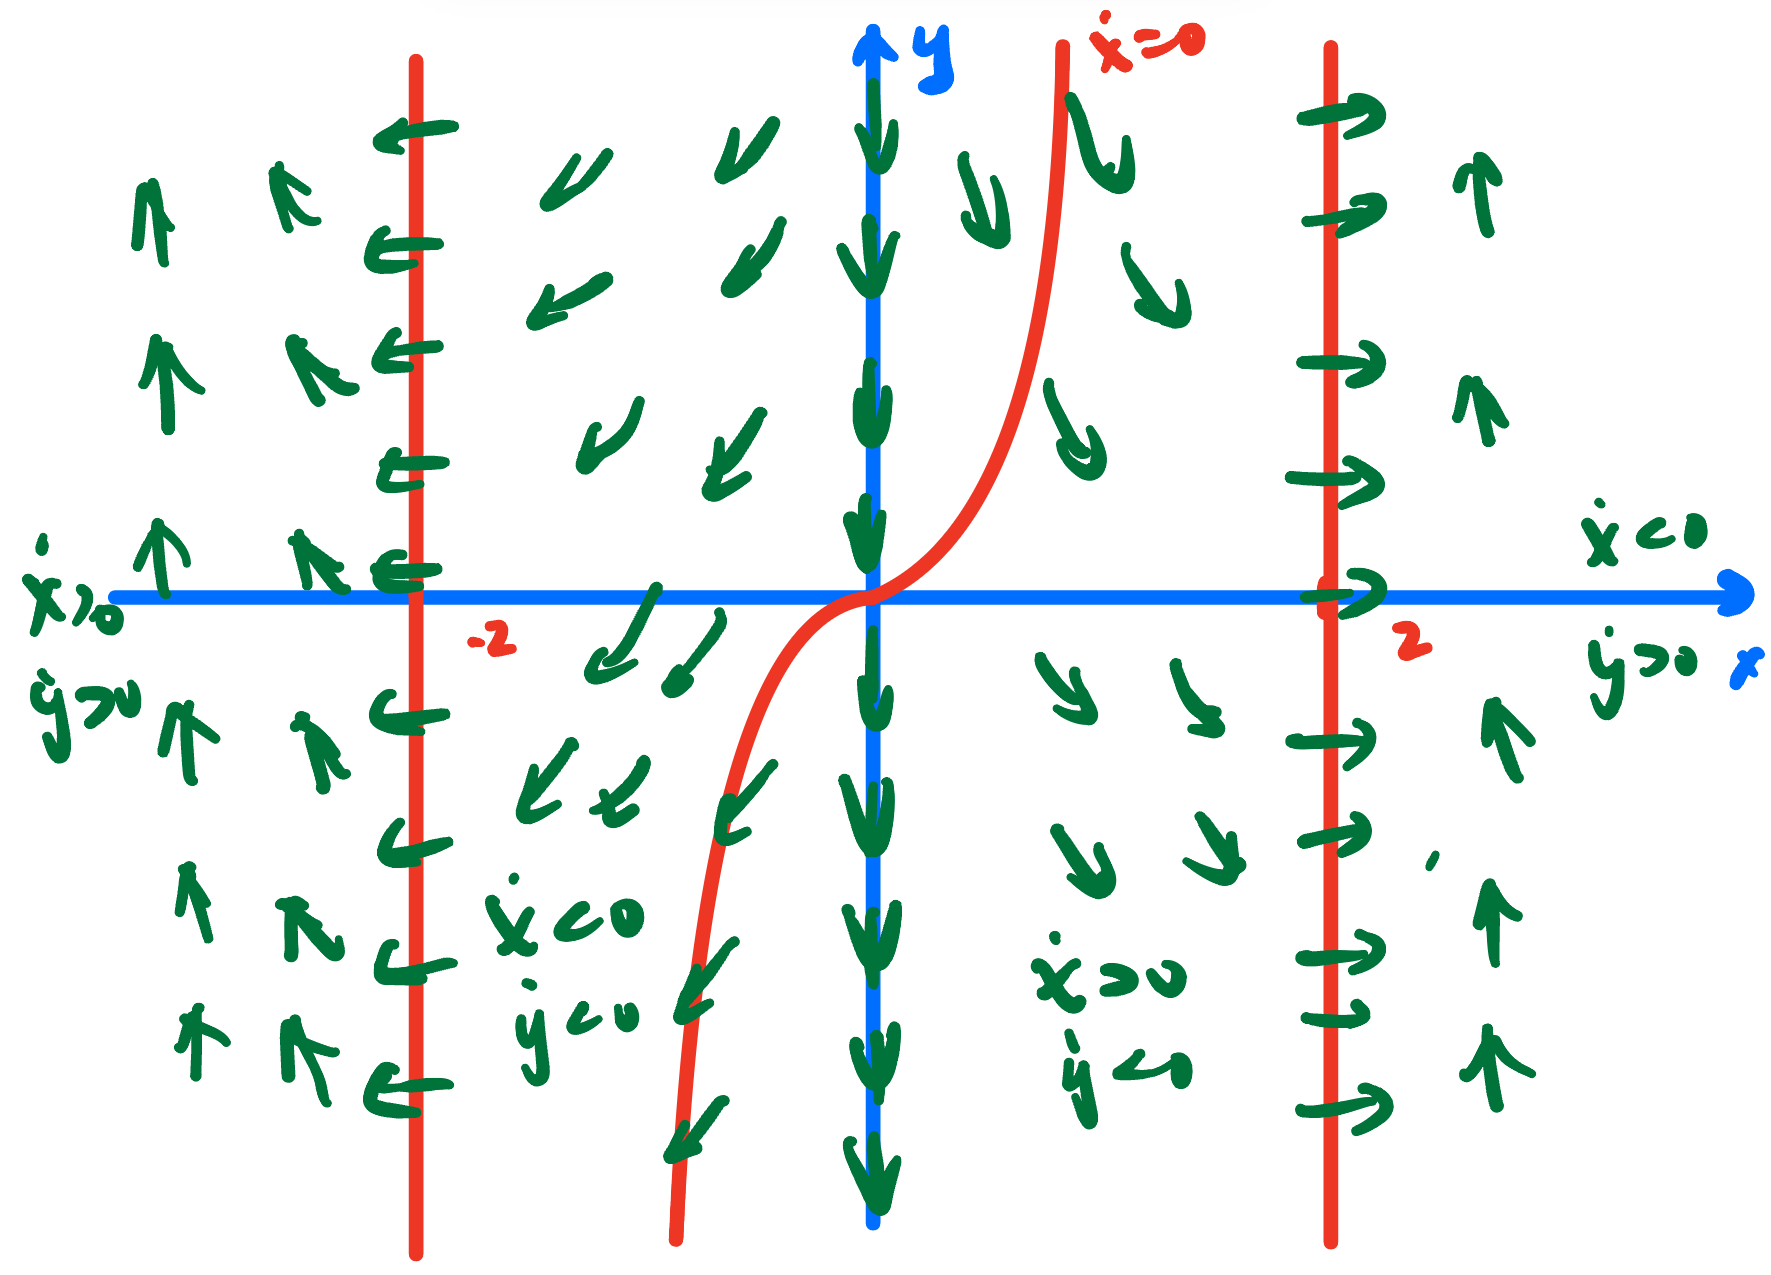
\includegraphics[width=0.7\linewidth]{3b.jpeg}
		\caption{Phase portrait of (b)}
		\label{fig:3b}
	\end{figure}

	When $b < 0 < \lambda$, the origin is unstable. The phase portrais below:
	\begin{figure}[H]
		\centering
		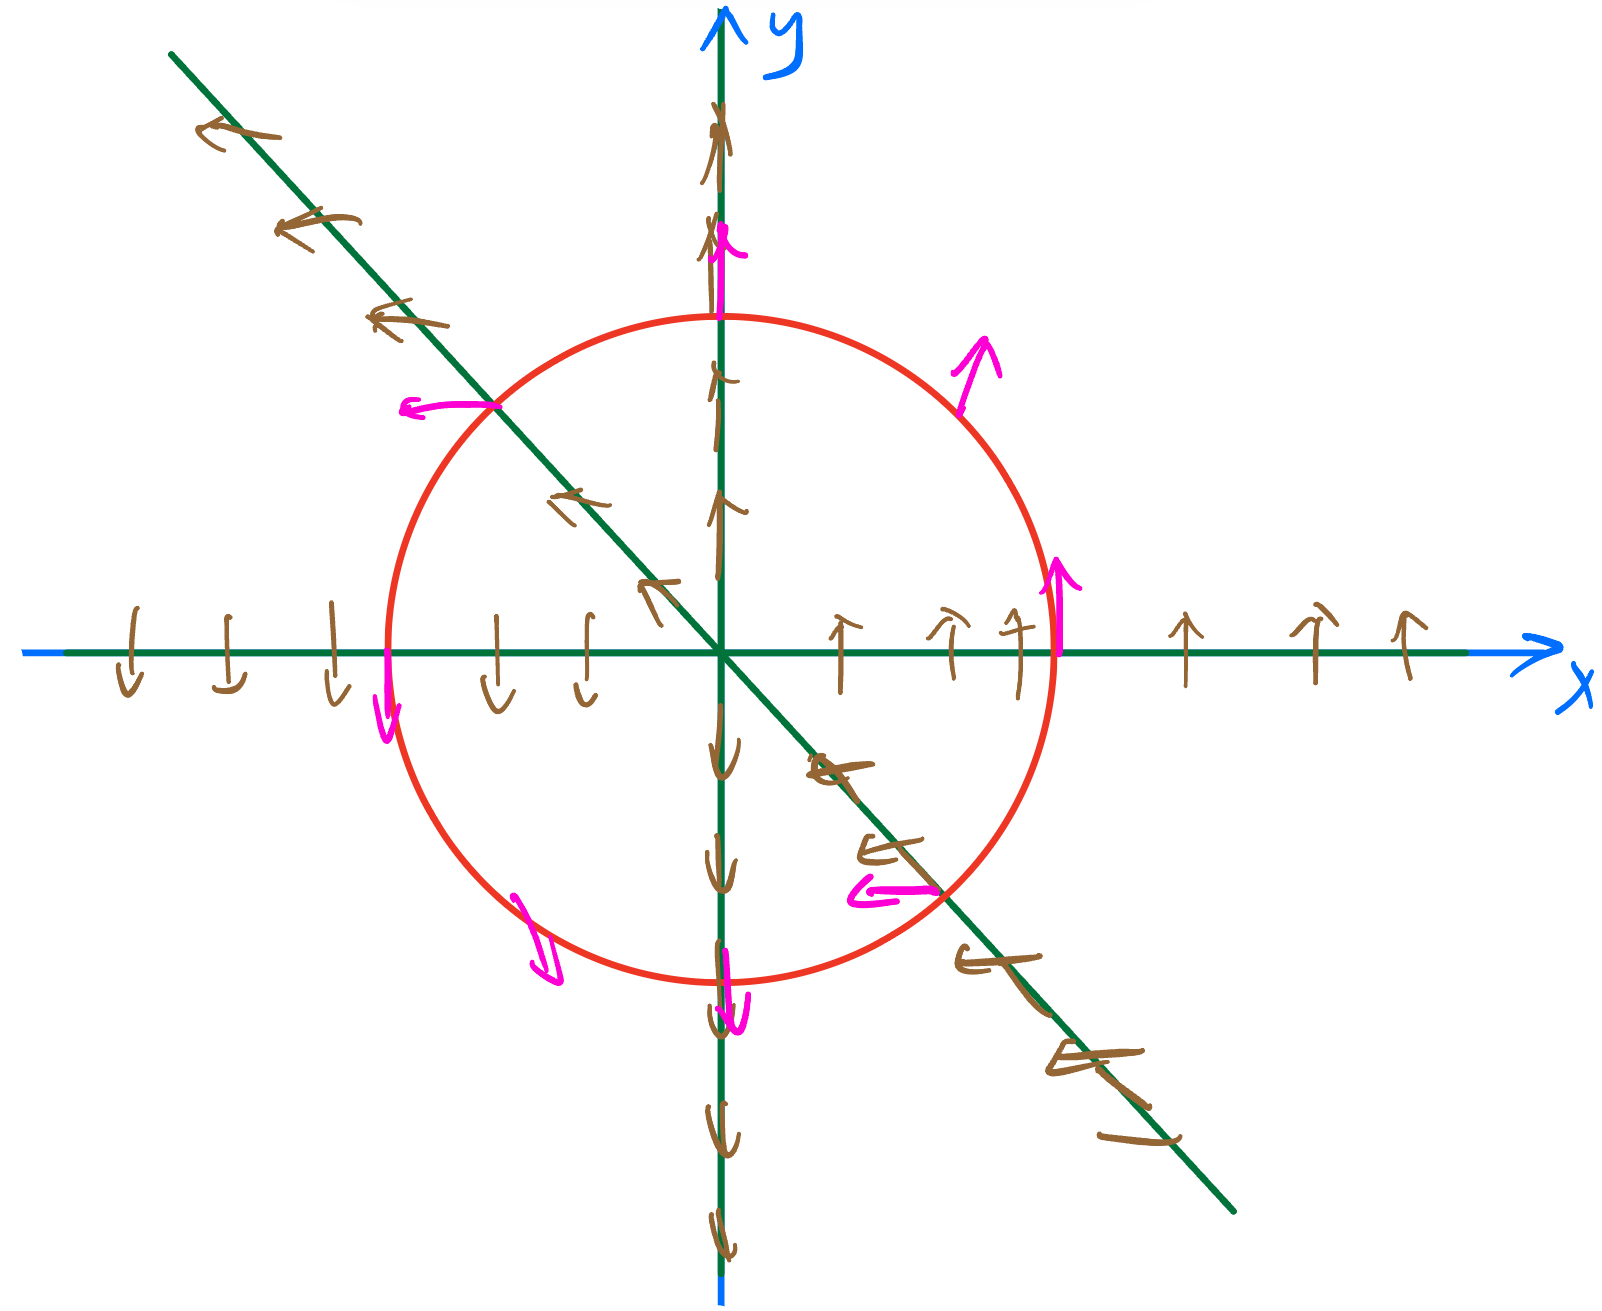
\includegraphics[width=0.7\linewidth]{3c.jpeg}
		\caption{Phase portrait of (c)}
		\label{fig:3c}
	\end{figure}

	When $b, \lambda > 0$, the origin is unstable. The phase portrais below:
	\begin{figure}[H]
		\centering
		\includegraphics[width=0.7\linewidth]{3d.jpeg}
		\caption{Phase portrait of (d)}
		\label{fig:3d}
	\end{figure}

\newpage
\section*{Problem 4}
For the damped harmonic oscillator, 
\[ m\ddot{x} + b\dot{x} + kx = 0 \]
where $m,b,k > 0$. 

\begin{enumerate}
	\item The equation can be written as two-dimensional system
	\[ \begin{cases}
		\dot{x} = y \\
		\dot{y} = -\frac{b}{m}y - \frac{k}{m}x \\
	\end{cases} \]

	So, the linear system is
	\[ \dot{\mathbf{x}} = \begin{bmatrix}
		0 & 1 \\
		-\frac{k}{m} & -\frac{b}{m} \\
	\end{bmatrix} \mathbf{x} \]

	\item To classify the fixed point, we need to find the eigenvalues of the matrix. The characteristic equation is 
	\[ \lambda^2 + \frac{b}{m}\lambda + \frac{k}{m} = 0 \]

	Now we know the eigenvalues are
	\[ \lambda_{1,2} = \frac{-b \pm \sqrt{b^2-4km}}{2m} \]

	So, the $\tau = \lambda_1 + \lambda_2 = -\frac{b}{m} < 0$, and $\Delta = \lambda_1 \lambda_2 = \frac{k}{m} > 0$. Since the fixed point has only one which is $(0, 0)$, we need to discuss the different cases of $\lambda_1$ and $\lambda_2$ for origin $(0,0)$.
	\newpage
	\begin{enumerate}
		\item When $b^2-4km < 0$, $\lambda_1, \lambda_2$ are complex conjugate. The origin is asymptotically stable and also a spiral, since the $\alpha < 0$ for all real part of eigenvalues.

			We can using Mathematica to plot the phase portrait and examine it below:
			\begin{figure}[H]
				\centering
				\includegraphics[width=0.5\linewidth]{3b_1.pdf}
				\caption{Phase portrait of system when $m=1, b=5, k=4$}
				\label{fig:3b_1}
			\end{figure}
		
		\item When $b^2-4km =0$, $\lambda_1, \lambda_2$ are real and identical. This is a degenrate node. We can draw the nullclines to determine it is stable at origin which is asymptotically stable.

			We can using Mathematica to plot the phase portrait and examine it below:
			\begin{figure}[H]
				\centering
				\includegraphics[width=0.5\linewidth]{3b_2.pdf}
				\caption{Phase portrait of system when $m=1, b=2, k=1$}
				\label{fig:3b_2}
			\end{figure}  
			
		\item When $b^2-4km > 0$, $\lambda_1, \lambda_2$ are real and distinct. The origin is asymptotically stable by referring the classification scheme diagram.

			We can using Mathematica to plot the phase portrait and examine it below:
			\begin{figure}[H]
				\centering
				\includegraphics[width=0.5\linewidth]{3b_3.pdf}
				\caption{Phase portrait of system when $m=1, b=4, k=2$}
				\label{fig:3b_3}
			\end{figure}




	\end{enumerate}
\end{enumerate}

\end{document}

